\documentclass{article}

\usepackage{graphicx}
%\usepackage{geometry}
\usepackage{placeins} % use float barriers
\usepackage{float}
\usepackage{subcaption}
\usepackage{longtable}
\usepackage[a4paper,margin=1in]{geometry}
\usepackage{grffile}
\usepackage{multirow}
\usepackage{siunitx}
\usepackage[table,xcdraw]{xcolor}

\title{RL experiment - widowx reach-v3}
\date{}

\begin{document}

\maketitle


%\begin{figure}[H]
%    \centering
%    \includegraphics[width=0.5\textwidth]{../reaching_jaco.jpg}
%\caption{The ReachingJaco-v1 environment}
%\end{figure}



\section{Introduction and methods}


The aim of this document is plot the results of the following RL experiment:

\begin{itemize}
  \item Algorithms: A2C, ACKTR, DDPG, PPO2, SAC, TD3, TRPO 
  \item Environment: widowx reach-v3
  \item Number of time steps: 1M
  \item Number of initialisation seeds: 2
  \item Number of parallel environments: 8 for ACKTR and PPO2 and 1 for SAC and TD3 (parallelisation not supported).
\end{itemize}


The performance metrics are defined as follows:

\begin{itemize}
  \item Train time (min) : Wall time to train.
  \item Success ratio : number of successful episodes / number of reachable episodes \\ 
An episode is successful if the distance between the finger tip and the target is less than or equal to 0.03. \\ 
  \item Average reaching time : sum (number of time steps of all successful episodes) /  number of successful episodes \\ 
An episode has a maximum of 100 time steps.
  \item Efficiency: mean reward / mean training walltime. 
\end{itemize}



\section{Results}

\subsection{Raw results}

%% GENERATED WITH https://www.tablesgenerator.com/
%% Please add the following required packages to your document preamble:
%% \usepackage[table,xcdraw]{xcolor}
%% If you use beamer only pass "xcolor=table" option, i.e. \documentclass[xcolor=table]{beamer}
%\begin{longtable}{l}
%\hline
%\begin{tabular}{llllll}
%exp type & {\color[HTML]{000000} mean reward} & {\color[HTML]{000000} mean train walltime (s)} & {\color[HTML]{000000} mean success ratio} & {\color[HTML]{000000} mean reach time} & {\color[HTML]{000000} efficiency (reward/s)} \\
%\hline
%A2C      & {\color[HTML]{000000} -243.73}     & {\color[HTML]{000000} 15.03}                   & {\color[HTML]{000000} 0}                  & {\color[HTML]{000000} }                & {\color[HTML]{000000} -16.21}                  \\
%ACKTR    & {\color[HTML]{000000} -238.09}     & {\color[HTML]{000000} 17.6}                    & {\color[HTML]{000000} 0}                  & {\color[HTML]{000000} }                & {\color[HTML]{000000} -13.53}                  \\
%DDPG     & {\color[HTML]{000000} -165.26}     & {\color[HTML]{000000} 21.58}                   & {\color[HTML]{000000} 0}                  & {\color[HTML]{000000} }                & {\color[HTML]{000000} -7.66}                   \\
%PPO2     & {\color[HTML]{000000} -264.8}      & {\color[HTML]{000000} 10.36}                   & {\color[HTML]{000000} 0}                  & {\color[HTML]{000000} }                & {\color[HTML]{000000} -25.56}                  \\
%SAC      & {\color[HTML]{000000} -242.1}      & {\color[HTML]{000000} 23.09}                   & {\color[HTML]{000000} 0}                  & {\color[HTML]{000000} }                & {\color[HTML]{000000} -10.49}                  \\
%TD3      & {\color[HTML]{000000} -184.24}     & {\color[HTML]{000000} 13.9}                    & {\color[HTML]{000000} 0}                  & {\color[HTML]{000000} }                & {\color[HTML]{000000} -13.25}                  \\
%TRPO     & {\color[HTML]{000000} -256.57}     & {\color[HTML]{000000} 16.05}                   & {\color[HTML]{000000} 0}                  & {\color[HTML]{000000} }                & {\color[HTML]{000000} -15.98}    \\   
%\hline          
%\end{tabular}
%\end{longtable}


\subsection{Learning curves}


\begin{figure}[H]
    \centering
    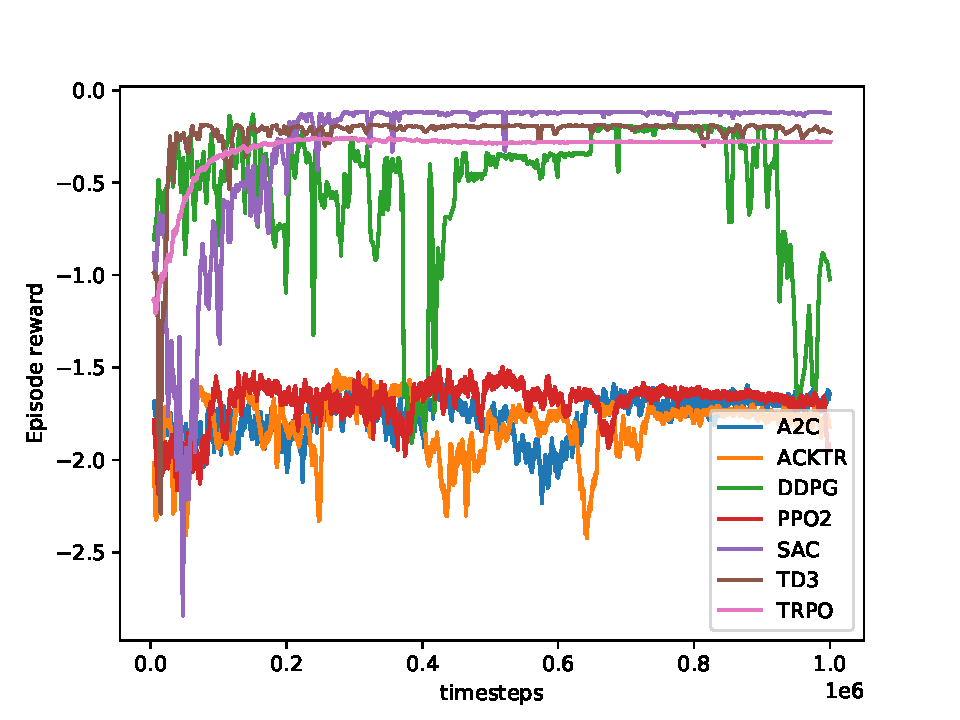
\includegraphics[width=0.7\textwidth]{../learning_curves.pdf}
\caption{All learning curves.}
\end{figure}


\begin{figure}[H]
    \centering
    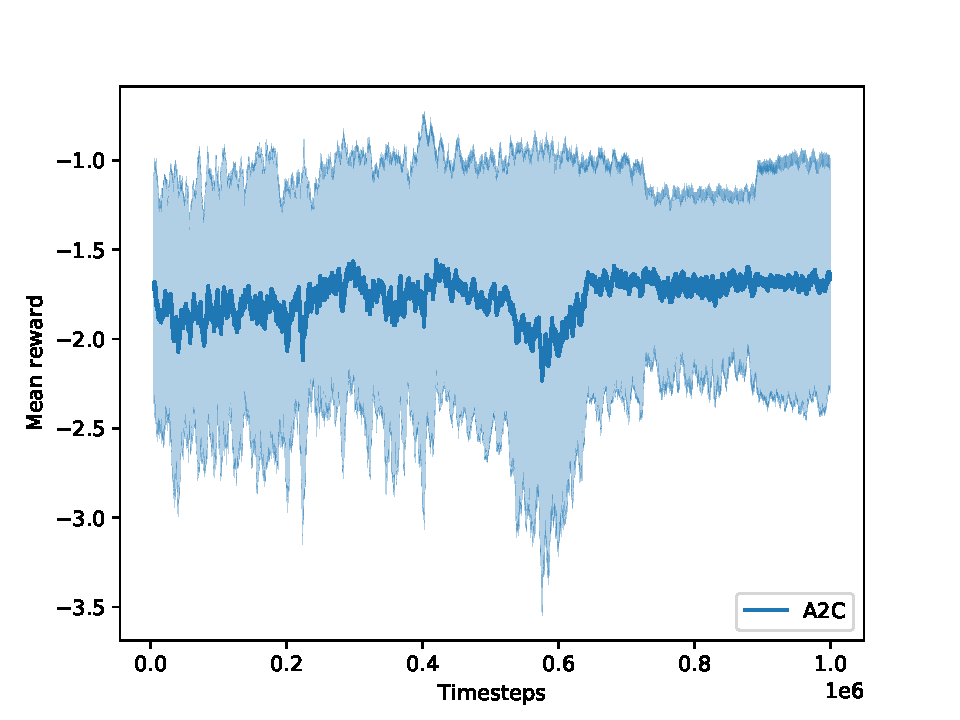
\includegraphics[width=0.7\textwidth]{../A2C.pdf}
\caption{Learning curve A2C.}
\end{figure}


\begin{figure}[H]
    \centering
    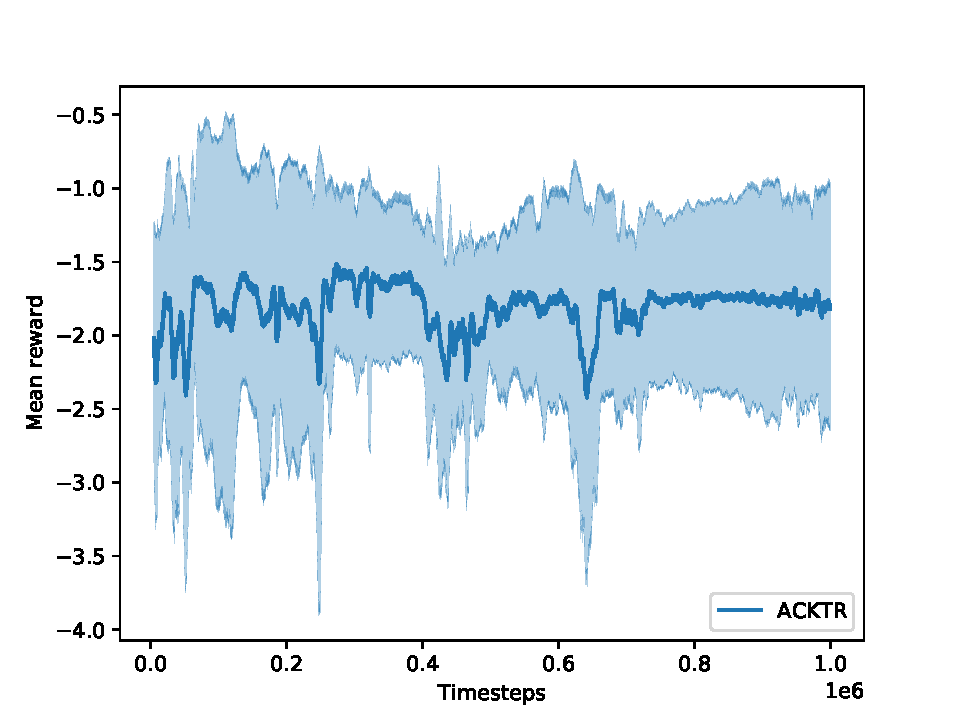
\includegraphics[width=0.7\textwidth]{../ACKTR.pdf}
\caption{Learning curve ACKTR.}
\end{figure}

\begin{figure}[H]
    \centering
    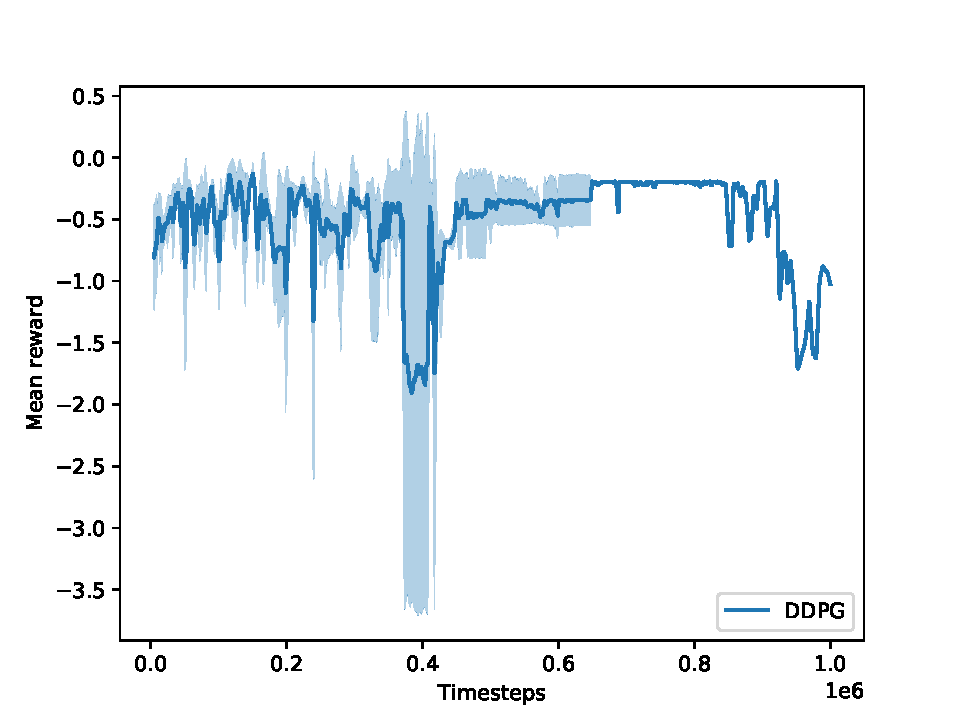
\includegraphics[width=0.7\textwidth]{../DDPG.pdf}
\caption{Learning curve DDPG.}
\end{figure}

\begin{figure}[H]
    \centering
    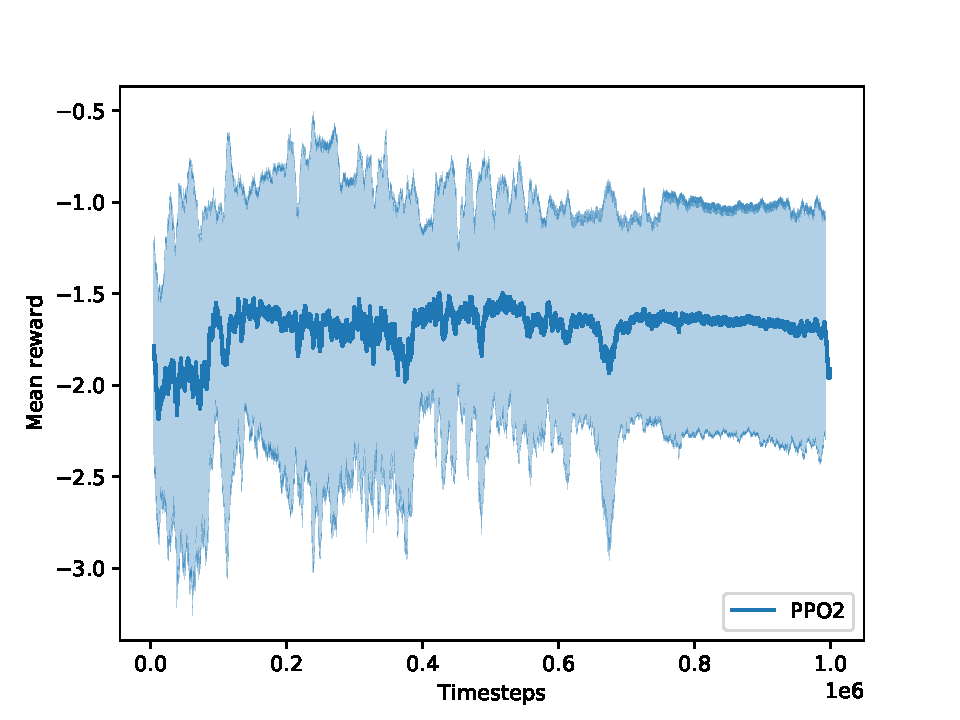
\includegraphics[width=0.7\textwidth]{../PPO2.pdf}
\caption{Learning curve PPO2.}
\end{figure}

\begin{figure}[H]
    \centering
    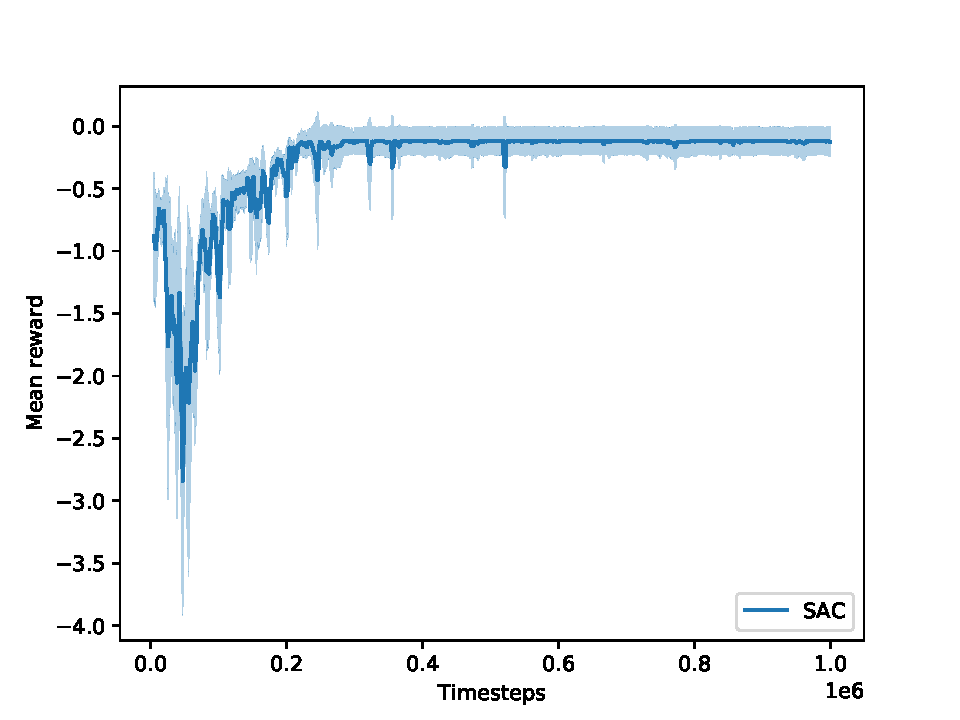
\includegraphics[width=0.7\textwidth]{../SAC.pdf}
\caption{Learning curve SAC.}
\end{figure}

\begin{figure}[H]
    \centering
    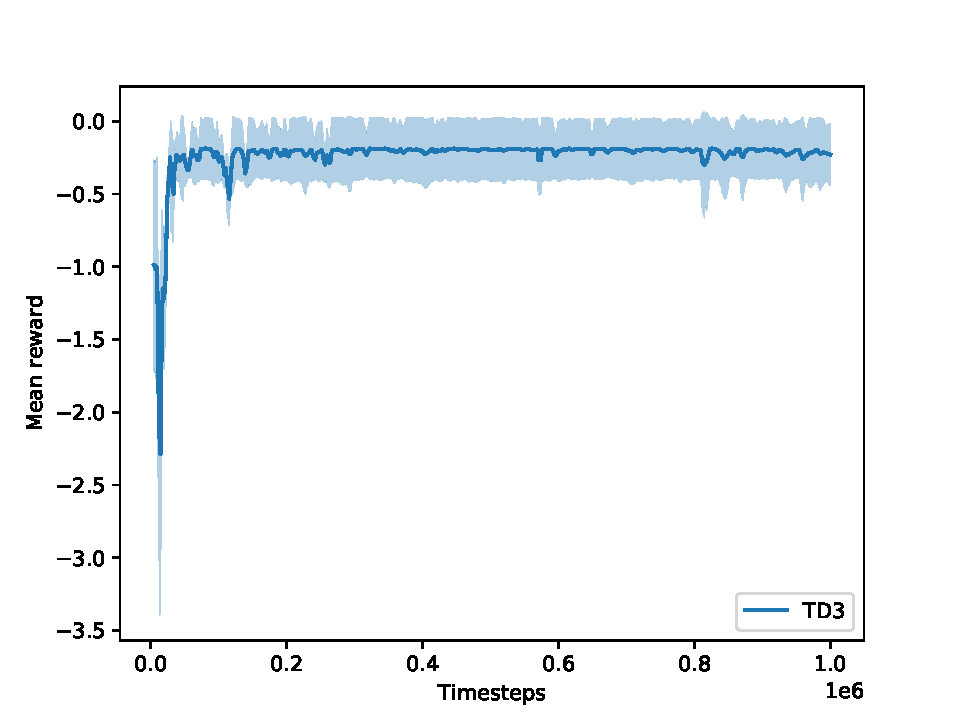
\includegraphics[width=0.7\textwidth]{../TD3.pdf}
\caption{Learning curve TD3.}
\end{figure}

\begin{figure}[H]
    \centering
    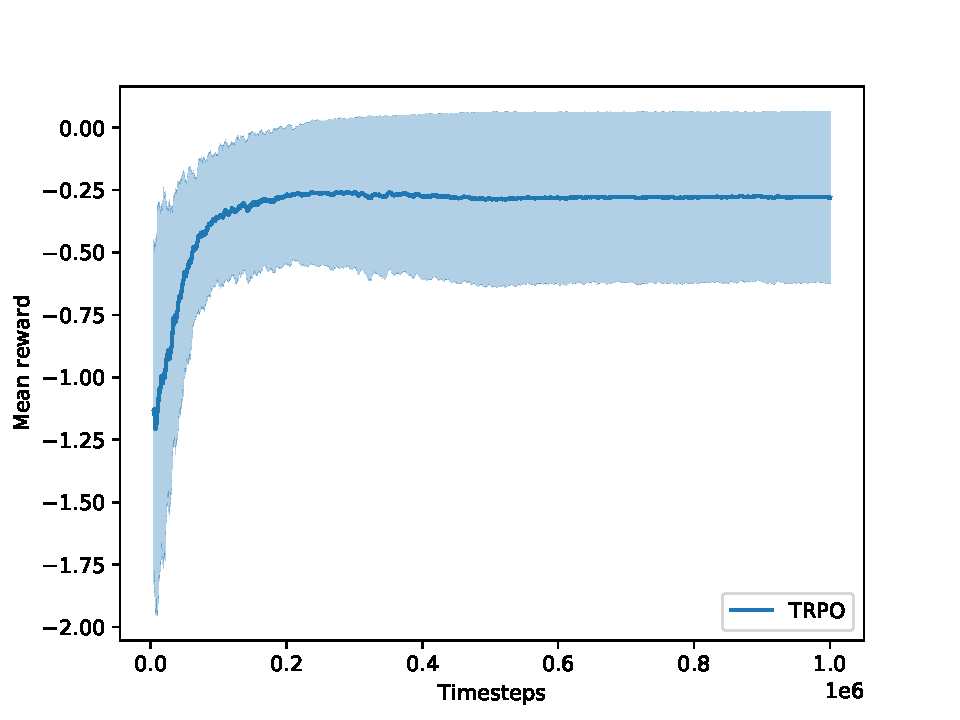
\includegraphics[width=0.7\textwidth]{../TRPO.pdf}
\caption{Learning curve TRPO.}
\end{figure}



\subsection{Evaluation}


\begin{figure}[H]
    \centering
    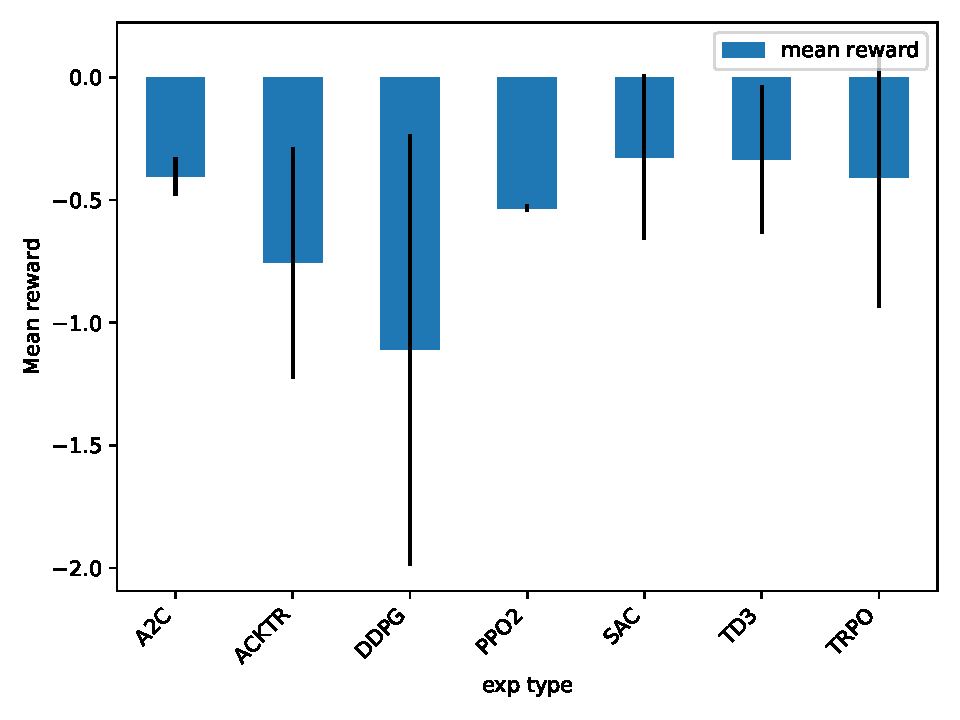
\includegraphics[width=0.7\textwidth]{../reward_by_exp_type.pdf}
\caption{Reward vs algorithms.}
\end{figure}



\begin{figure}[H]
    \centering
    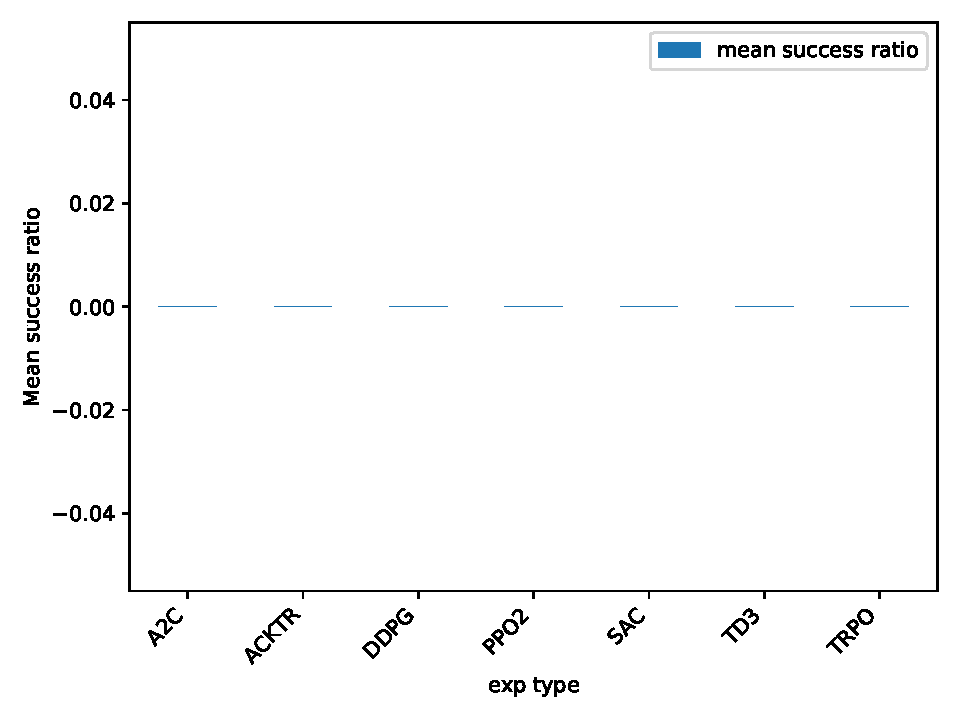
\includegraphics[width=0.7\textwidth]{../success_by_exp_type.pdf}
\caption{Success ratio vs algorithms.}
\end{figure}


\begin{figure}[H]
    \centering
    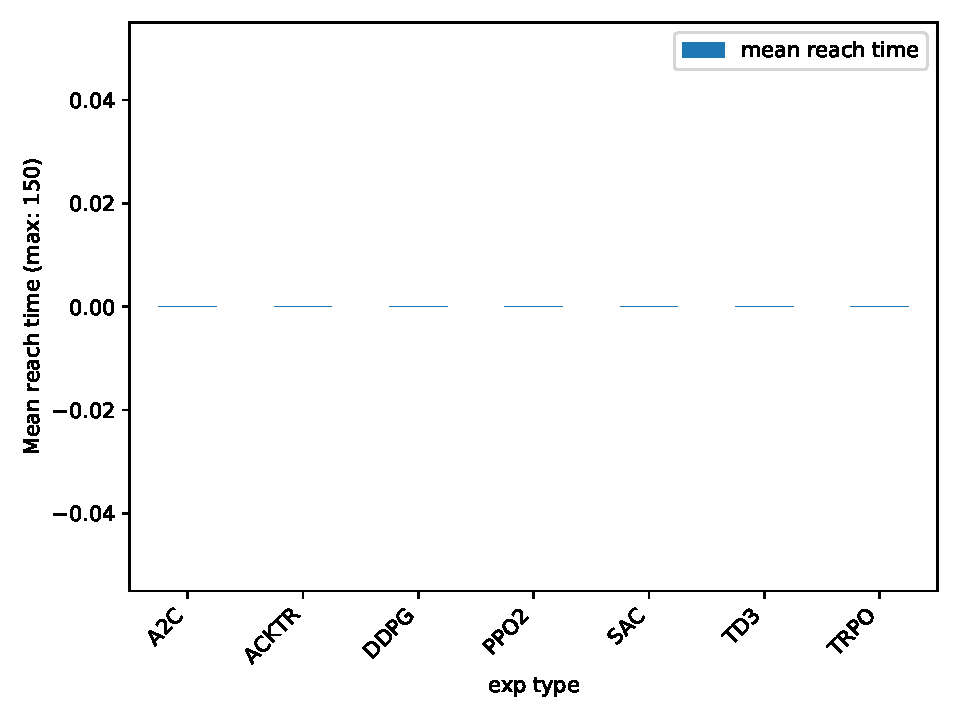
\includegraphics[width=0.7\textwidth]{../reachtime_by_exp_type.pdf}
\caption{Reach time vs algorithms.}
\end{figure}



\begin{figure}[H]
    \centering
    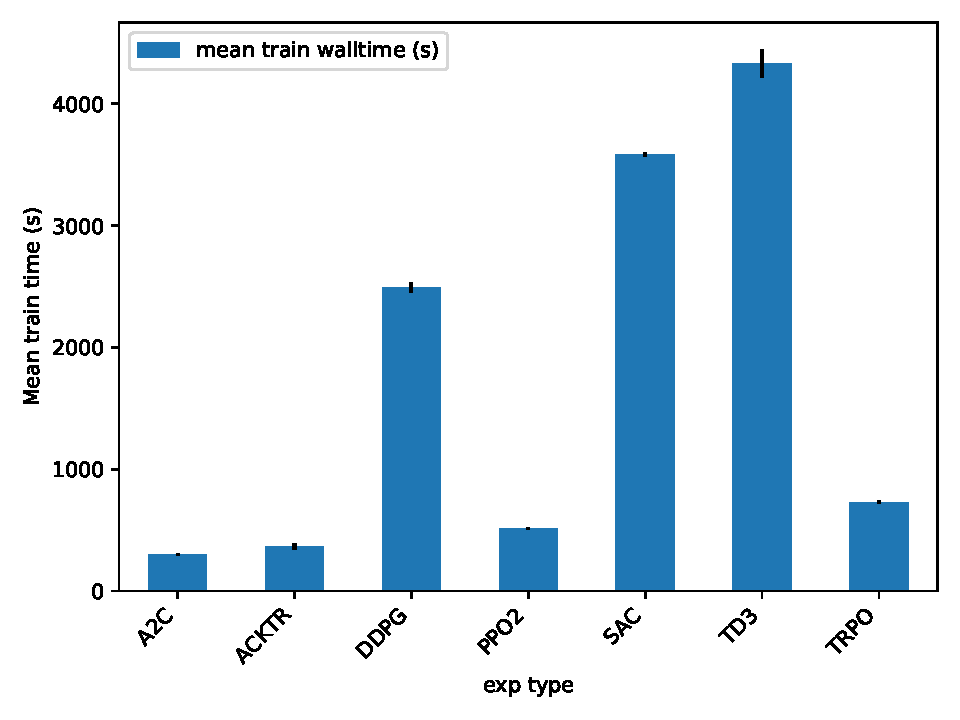
\includegraphics[width=0.7\textwidth]{../walltime_by_exp_type.pdf}
\caption{Train walltime vs algorithms.}
\end{figure}




\section{Findings summary}


%\begin{itemize}
%  \item With the default hyperparameters, TD3 showed the best training efficiency and the best return.
%  \item From the shape of the training curve, ACKTR and PPO2 could benefit from a longer training.
%  \item After training, the arm is moving towards the target. However, none of the trained model successfully reached the target within the distance threshold of 0.03.
%  \item TD3 and SAC are the longest lgorithms to train (due to parallelisation not being supported).
%  \item A budget of 0.01M timesteps is not enough to obtain a satisfactory hyperparameter tuning. 0.1M timesteps were enough.
%\end{itemize} 



\end{document}